% xetex compatible variant that support TTF fonts according to company rules
\documentclass[ignorenonframetext, professionalfonts, hyperref={unicode}]{beamer}

\usetheme{Epam}

\usepackage{fontspec}
\setsansfont{SourceSansPro-Regular}
%\setbeamerfont{frametitle}{family=\fontspec{Oswald}}
\setbeamerfont{frametitle}{family=\fontspec{Oswald}}
\setbeamerfont{block title}{family=\fontspec{Oswald}}

%\setmainfont{Times New Roman}
\defaultfontfeatures{Mapping=tex-text}
\defaultfontfeatures{Ligatures=TeX}

%\setsansfont{Arial}
%\setromanfont{Trebuchet MS}

\usepackage{cmap}
\usepackage{graphicx}

\usepackage{textcomp}

\usepackage{beamerthemesplit}

\usepackage{ulem}

\usepackage{verbatim}
\usepackage{import}

\usepackage{listings}
\lstloadlanguages{bash}

\lstset{escapechar=`,
	captionpos=b,
	extendedchars=false,
	language=sh,
%	frame=single,
	tabsize=2, 
	columns=fullflexible, 
%	basicstyle=\scriptsize,
	keywordstyle=\color{blue}, 
	commentstyle=\itshape\color{brown},
%	identifierstyle=\ttfamily, 
	stringstyle=\mdseries\color{green}, 
	showstringspaces=false, 
	numbers=left, 
	numberstyle=\footnotesize, 
	breaklines=true, 
	inputencoding=utf8,
	keepspaces=true,
	morekeywords={u\_short, u\_char, u\_long, in\_addr}
	}

\definecolor{darkgreen}{cmyk}{0.7, 0, 1, 0.5}

\lstdefinelanguage{diff}
{
    morekeywords={+, -},
    sensitive=false,
    morecomment=[l]{//},
    morecomment=[s]{/*}{*/},
    morecomment=[l][\color{darkgreen}]{+},
    morecomment=[l][\color{red}]{-},
    morestring=[b]",
}

\author[Epam]{{\bf Epam}\\Low Level Programming Department}

%\institution[EPAM]{EPAM}
%\logo{\includegraphics[width=1cm]{logo.png}}

\graphicspath{{../../slides/cmdline/clipart/}{../../slides/bash/clipart/}}

\bibliographystyle{unsrt}
\setbeamertemplate{bibliography item}{\insertbiblabel}

\AtBeginSection[]{%
  \begin{frame}<beamer>
    \frametitle{}
    \tableofcontents[
        sectionstyle=show/shaded, hideallsubsections ]
  \end{frame}
  \addtocounter{framenumber}{-1}% If you don't want them to affect the slide number
}

% \regex for regular expressions
\newcommand{\regex}[1]{ %
\expandafter{$\ulcorner{\color{blue}\texttt{#1}}\lrcorner$} %
}



\title{Введение в GNU/Linux}


%%%%%%%%%%%%%%%%%%%%%%%%%%%%%%%%%%%%%%%%%%%%%%%%%
%%%%%%%%%% Begin Document  %%%%%%%%%%%%%%%%%%%%%%
%%%%%%%%%%%%%%%%%%%%%%%%%%%%%%%%%%%%%%%%%%%%%%%%%




\begin{document}

\begin{frame}
	\frametitle{}
	\titlepage
	\vspace{-0.5cm}
	\begin{center}
	%\frontpagelogo
	\end{center}
\end{frame}


%%%%%%%%%%%%%%%%%%%%%%%%%%%%%%%%%%%%%%%%%   
%%%%%%%%%% Content starts here %%%%%%%%%%
%%%%%%%%%%%%%%%%%%%%%%%%%%%%%%%%%%%%%%%%%



\section{Working with text data}

\subsection{Text editors and filters}
\mode<all>{\begin{frame}{Текст в Unix}
  В Unix (и Linux) в виде обычного текста или \alert{plain text} представлены:\pause
  \begin{itemize}
    \item \alert{конфигурационные файлы}, как локальные\footnote{в каталоге \$HOME} , так и общесистемные\footnote{в каталоге /etc} \pause
    \item \alert{системные логи}\footnote{справедливо для \alert{syslog} и совместимых систем}
    \item \alert{исходные тексты программ}, включая скрипты на Shell
    \item \alert{основной формат ввода и (или) вывода данных} для множества программ и утилит
  \end{itemize} 

\end{frame}


%\begin{frame}{Просмотр обычных файлов}
%  \begin{itemize}
%    \item Просмотр текста:
%      \begin{itemize} 
%        \item \alert{cat} - вывести на stdout\footnote{Для двоичных файлов: чревато порчей настроек терминала} \pause
%        \item \alert{more} - вывести, разбив на страницы
%        \item \alert{less}\footnote{может отсутствововать в стандартной поставке} - \alert{more} на стероидах, с прокруткой, поиском
%      \end{itemize} \pause
%    \item Просмотр двоичных данных:
%      \begin{itemize} 
%        \item \alert{od} - дамп файла в не-текстовых форматах
%\lstinputlisting[frame=single,basicstyle=\tiny]{../../sam-solutions/samples/od}
%        \item \alert{strings} - извлечь текстовые строки из двоичных файлов
%      \end{itemize}
%  \end{itemize}
%
%\end{frame}
%

%\begin{frame}{Редакторы}
%
%  \begin{itemize}
%    \item  Любой редактор, с которым вы можете справится. \pause Но его может не быть в вашей системе\ldots \pause
%    \item Редактор \alert{vi} присутствует как стандартный в любой Unix-подобной системе\footnote{В этом качестве он внесен в стандарт Single Unix Specification. Существует множество реализаций редакторов, совместимых c vi: vim, elvis, nvi, vi-mode в Emacs, Sublime Text 2, vi из busybox и т.д.} \pause
%    \item Не обязательно редактировать локально: В \alert{mc}, \alert{vim}, \alert{emacs} есть возможность удалённого редактирования файлов\footnote{С получением и сохранением данных по протоколу FTP и SSH}.
%  \end{itemize}
%
%\end{frame}
%
%\begin{frame}{vi и vim}
%  Перед стартом:
%
%  \begin{enumerate}
%    \item  Редактор vi изначально создавался как универсальный и переносимый\footnote{Обязан работать на любых типах терминалов и виртуальных консолей}. Все действия можно осуществить на алфавитно-цифровой части клавиатуры, без мыши. \pause
%    \item \alert{Редактор командного стиля}\footnote{Командного стиля, а не меню-ориентированный}. Действия подачей прямых управляющих команд. \pause \newline
%      3 основных режима: \sout{портить текст и противно бибикать}
%      \begin{itemize}
%        \item[-] \alert{Командный режим} (Normal mode) - по умолчанию при запуске.
%        \item[-] \alert{Режим изменения текста} (Edit mode)
%        \item[-] \alert{Режим построчного редактирования} (Ex mode) - операции над файлом целиком\footnote{сохранение, открытие файлов, выход, вставка файла в текущий и т.д.}.
%      \end{itemize}
%  \end{enumerate} \pause
%  \alert{Упражнение}: проходим \alert{vimtutor}, встроенный в vim учебник\footnote{ export LANG='ru\_RU.UTF-8' - на русском языке }
%\end{frame}

\begin{frame}{Текстовый фильтр}

  Определение:\newline \alert{Текстовый фильтр} - программа, обрабатывающая и преобразующая текст. \newline

  Примеры: \alert{sort}, \alert{uniq}, \alert{cut}, \alert{grep} \pause
  \begin{itemize}
    \item Фильтр, запущенный без параметров - читает стандартный ввод.
    \item Параметры фильтра - интерпретируются как имена файлов
    \item Ключи фильтра - управляют режимами работы
  \end{itemize} \pause

  Фильтр почти всегда используется совместно с перенаправлением ввода-вывода Shell (особенно '|', pipes). cmd1 | cmd2

\end{frame}

\begin{frame}{Простые текстовые фильтры}

  Соглашения о параметрах: \alert{'-'} как имя файла обозначает стандартный ввод.

  \begin{itemize}
    \item \alert{cat} и \alert{tac} - вывести файл целиком \pause
    \item \alert{head} и \alert{tail} - вывести начало и конец файла \pause
    \item \alert{sort} и \alert{uniq} - сортировка и убрать повторы в отсортированном \pause
    \item \alert{paste} - объединить файлы построчно \pause
    \item \alert{wc} - счётчик строк, слов и байт в тексте \pause
    \item \alert{tee} - копирует стандартный ввод в файл и на экран
    \item \alert{grep} - поиск по образцу \pause

  \end{itemize}
\end{frame}

%\begin{frame}{Регулярные выражения}
%
%  \begin{block}{Как описать текст?}
%    Необходим инструмент и формат описания текста
%  \end{block} \pause

%  \begin{block}{Регулярные выражения}
%    \alert{Регулярные выражения (regular expression или regexp)} -  специальные строки символов, которые задаются для поиска совпадающих фрагментов. Иначе говоря это способ описания наборов букв.
%  \end{block} \pause
%
%  \begin{block}{Универсальный язык описания текста}
%    Все Unix-программы, осуществляющие поиск в тексте, используют регулярные выражения.
%  \end{block}
%
%\end{frame}
%
%\begin{frame}[fragile]{Элементы регулярных выражений}
%    \begin{itemize}
%      \item \alert{литералы} - обычные символы (буквы и цифры) \pause
%      \item \alert{метасимволы} - спецсимволы (количество повторов, группировка фрагментов, позиция в тексте).
%    \end{itemize} \pause
%
%    Примеры регулярных выражений:\newline
%\begin{lstlisting}
%~$ file /bin/* | grep symbolic
%~$ grep -o 'user[0-9]*' /var/log/auth.log
%\end{lstlisting}
%\end{frame}
%
%%\subsection{Метасимволы}
%\begin{frame}{Класс на 1 символ}
%  \begin{itemize}
%    \item \alert{.} (точка)  - заменяет любой символ \newline
%      Пример: \regex{us.r.} = 'user0', 'us rX', 'us9r ' и т.д. \pause
%    \item \alert{[ ]} символьный класс - заменяет любой символ из перечисленных в скобках
%      \begin{enumerate}
%        \item \regex{user[0-9]} = 'user0', 'user5', но не равно 'user'
%        \item \regex{-[abc-]} = '--', '-a', '-b', '-c', но не равно '--a'
%        \item \regex{[\textasciicircum{}abc]1}\footnote{инвертировать символьный класс} = 'd1', '11', но не равно 'a1'
%      \end{enumerate} \pause
%    \item \alert{[:class:]} - дополнительные POSIX-классы для символов, \alert{внутри символьного класса}\footnote{Да, на редкость уродливый синтаксис} \newline
%        Примеры классов: \alert{[:alnum:]}, \alert{[:alpha:]} \alert{[:digit:]} \alert{[:space:]} \alert{[:lower:]}, \alert{[:upper:]}, \alert{[:print:]} \newline
%        Примеры regexp с POSIX классами: \regex{[ы[:digit:]]}
%  \end{itemize}
%\end{frame}
%
%
%\begin{frame}[fragile]{квантификаторы - регулируем повторы}
%
%  \alert{Квантификаторы} указывают, сколько раз может повторяться символ или выражение, после которого указаны.  Не являются шаблонами текста.
%
%  \begin{itemize}
%    \item \alert{?} - необязательный символ \newline
%      пример: \regex{a.?b} - совпадёт с 'ab', 'a9b', 'a b' \pause
%    \item \alert{*} - любое количество символов, включая нулевое \newline
%      примеры: \regex{.*}, \regex{[[:digit:]]*} \pause
%    \item \alert{+} - не менее одного символа \newline
%      примеры: \regex{[a-d]+}, \regex{(02:)+}
%  \end{itemize}
%\end{frame}
}
\mode<all>{\begin{frame}[fragile]{Разбираем пример использования фильтров.}
  \begin{block}{Cчитаем участников тренинга используя текстовые фильтры.}
\begin{lstlisting}
cat /tmp/chat # посмотреть содержимое
cat /tmp/chat | grep AM # строки со временем AM
cat /tmp/chat | grep -e AM -e PM # строки со временем AM и PM
grep -e AM -e PM /tmp/chat | sort # сортируем
grep -e AM -e PM /tmp/chat | sort | cut -f 1,2 -d ' ' # оставить имя фамилия
grep -e AM -e PM /tmp/chat | sort | cut -f 1,2 -d ' ' | uniq # удалить дубликаты
grep -e AM -e PM /tmp/chat | sort | cut -f 1,2 -d ' ' | uniq | wc -l # считаем строки 
\end{lstlisting}
  \end{block} 
\end{frame}
} 
\mode<all>{\begin{frame}{Простые текстовые фильтры}

  Соглашения о параметрах: \alert{'-'} как имя файла обозначает стандартный ввод.
  

  \begin{itemize}
    \item \alert{cat} и \alert{tac} - вывести файл целиком
    \item \alert{head} и \alert{tail} - вывести начало и конец файла 
    \item \alert{sort} и \alert{uniq} - сортировка и убрать повторы в отсортированном
    \item \alert{paste} - объединить файлы построчно
    \item \alert{wc} - счётчик строк, слов и байт в тексте
    \item \alert{grep} - поиск по образцу

  \end{itemize}
\end{frame}
} 
\mode<all>{\begin{frame}{Текстовые редакторы}
	\begin{itemize}
		\item Интерактивные
			\begin{itemize}
				\item vi
				\item vim
				\item emacs
			\end{itemize}
		\item Поточные
			\begin{itemize}
				\item {\tt ed}
				\item {\tt sed}
				\item {\tt awk}
			\end{itemize}
	\end{itemize}
\end{frame}

%%\begin{frame}[fragile]{Метасимволы}
%	\begin{block}{grep, sed, awk}
%	\end{block}
%	\begin{itemize}
%		\item {\tt .} -- любой символ за исключением пустой строки
%		\item {\tt *} -- любоe количество символов, которые стоят перед {\tt *}
%		\item {\tt \^{}} -- начало строки
%		\item {\tt \$} -- конец строки
%		\item {\tt [...]} -- любой символ из заключенных в скобки
%	\end{itemize}
%\end{frame}

\begin{frame}[fragile]{sed}
	\begin{block}{Сценарии}
		{\tt [ addr [ ,  addr ] ] cmd [ args ]}
	\end{block}

	\tiny
	\begin{block}{Команды}
		\begin{itemize}
		  \item {\tt d} -- удалить строку
			  \begin{verbatim} who | sed -e '2,4 d' \end{verbatim}
			  \begin{verbatim} who | sed -e '/pts/ d' \end{verbatim}
		  \item {\tt s} -- замена по регулярному выражению
			  \begin{verbatim} who | sed -e "s/USER/user/g" \end{verbatim}
		  \item {\tt a, i} -- добавить строку после (перед) текущей
			  \begin{verbatim} who | sed -e 'a Text' \end{verbatim}
		\end{itemize}
	\end{block}
%	\pause
%	\begin{block}{Задача}
%		С помощью {\tt find} найти все вложенные директории в {\tt /etc} и 
%		''переделать'' их в windows-style
%	\end{block}
\end{frame}
}
%\mode<all>{
\begin{frame}{Регулярные выражения}

  \begin{block}{Как описать текст?}
    Необходим инструмент и формат описания текста
  \end{block} \pause

  \begin{block}{Регулярные выражения}
    \alert{Регулярные выражения (regular expression или regexp)} -  специальные строки символов, которые задаются для поиска совпадающих фрагментов. Иначе говоря это способ описания наборов букв.
  \end{block} \pause

  \begin{block}{Универсальный язык описания текста}
    Все Unix-программы, осуществляющие поиск в тексте, используют регулярные выражения.
  \end{block}

\end{frame}

\begin{frame}[fragile]{Элементы регулярных выражений}
    \begin{itemize}
      \item \alert{литералы} - обычные символы (буквы и цифры) \pause
      \item \alert{метасимволы} - спецсимволы (количество повторов, группировка фрагментов, позиция в тексте).
    \end{itemize} \pause

    Примеры регулярных выражений:\newline
\begin{lstlisting}
~$ file /bin/* | grep symbolic
~$ grep -o 'user[0-9]*' /var/log/auth.log
\end{lstlisting}
\end{frame}

%\subsection{Метасимволы}
\begin{frame}{Класс на 1 символ}
  \begin{itemize}
    \item \alert{.} (точка)  - заменяет любой символ \newline
      Пример: \regex{us.r.} = 'user0', 'us rX', 'us9r ' и т.д. \pause
    \item \alert{[ ]} символьный класс - заменяет любой символ из перечисленных в скобках
      \begin{enumerate}
        \item \regex{user[0-9]} = 'user0', 'user5', но не равно 'user'
        \item \regex{-[abc-]} = '\textendash\textendash', '-a', '-b', '-c'
        \item \regex{[\textasciicircum{}abc]1}\footnote{инвертировать символьный класс} = 'd1', '11', но не равно 'a1'
      \end{enumerate} \pause
    \item \alert{[:class:]} - дополнительные POSIX-классы для символов, \alert{внутри символьного класса}\footnote{Да, на редкость уродливый синтаксис} \newline
        Примеры классов: \alert{[:alnum:]}, \alert{[:alpha:]} \alert{[:digit:]} \alert{[:space:]} \alert{[:lower:]}, \alert{[:upper:]}, \alert{[:print:]} \newline
        Примеры regexp с POSIX классами: \regex{[ы[:digit:]]}
  \end{itemize}
\end{frame}


\begin{frame}[fragile]{квантификаторы - регулируем повторы}

  \alert{Квантификаторы} указывают, сколько раз может повторяться символ или выражение, после которого указаны.  Не являются шаблонами текста.

  \begin{itemize}
    \item \alert{?} - необязательный символ \newline
      пример: \regex{a.?b} - совпадёт с 'ab', 'a9b', 'a b' \pause
    \item \alert{*} - любое количество символов, включая нулевое \newline
      примеры: \regex{.*}, \regex{[[:digit:]]*} \pause
    \item \alert{+} - не менее одного символа \newline
      примеры: \regex{[a-d]+}, \regex{(02:)+}
  \end{itemize}
\end{frame}
} % to video

\section{Search and process files with find}
\mode<all>{\begin{frame}[fragile]{Файловая система. Данные и метаданные.}
    \begin{columns}
        \column{0.6\textwidth}
  \begin{block}{Упражнение. Выполнить команды. Расскажите что получили.}
    cat /etc/passwd
    \break
    stat /etc/passwd
  \end{block} 
        \column{0.3\textwidth}
        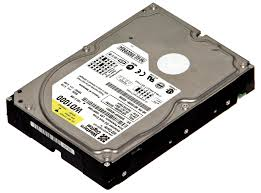
\includegraphics[height=3cm]{hw_hdd.jpg} 
    \end{columns}
\pause
Матаданные - информация о файле.
\begin{itemize}
 \item Размер файла
 \item Владелец и права доступа 
 \item Время доступа, изменения
\end{itemize}
\end{frame}
}
\mode<all>{\begin{frame}[fragile]{Поиск файлов командой find}
    \alert{find} ищет файлы в заданной директории и производит над ним заданную операцию.
	\begin{block}{Часто используемые параметры поиска}
		\begin{itemize}
			\item {\tt -name}, {\tt -iname} -- имя файлового объекта, включая метасимволы 
			\item {\tt -type} -- тип файлового объекта
			\item {\tt -size} -- размер [cwbkMG]
			\item {\tt -perm} -- права доступа
			\item {\tt -user} -- владелец
			\item {\tt ...} -- другие опции man find 
		\end{itemize}
	\end{block}
\end{frame}

\begin{frame}[fragile]{Файлы найдены}
	\begin{block}{Действия над результом поиска}
		\begin{itemize}
			\item {\tt -print} -- вывод на stdout (по умолчанию)
			\item {\tt -printf} -- форматированный вывод
			\item {\tt -exec} -- выполнить команду
			\item {\tt -ls} -- замена -exec ls -l \{\} ;
			\item {\tt -delete} -- удалить файл
		\end{itemize}
	\end{block}
\end{frame}

\begin{frame}[fragile]{Примеры использования команды find}
            В текущей директории найти все файлы *.o и вывести на экран 
            \begin{verbatim} find . -name '*.o' -print \end{verbatim}
            \begin{verbatim} find -name '*.o' \end{verbatim}
            Поск по типу и владельцу файла.
            \begin{verbatim} find -type d -user altlinux \end{verbatim}
            Составная команда, множество условий
            \begin{verbatim} find /root \( -name '*.pyc' -o -name '*.py' \) \
-type f -user root -size +300k -size -1024k \
-exec ls -l \{\} \; \end{verbatim}
 Дополнительно: позволяет преодолеть лимит на кол-во аргументов в командной строке. 
 \textquotedblleft Arguments too long.\textquotedblright 
\end{frame}

\begin{frame}[fragile]{xargs}
			Утилита для создания и запуска команд из стандартного потока ввода:
		\begin{verbatim}
xargs [options] command [command options]
                \end{verbatim}
		\begin{itemize}
			\item {\tt -d} -- разделитель
			\item {\tt -0} -- null-terminated строки
			\item {\tt -I text} -- подстановка
			\item {\tt -n N} -- максимальное количество аргументов
			\item {\tt -P N} -- максимальное количество процессов
		\end{itemize}

%Для работы с разделителями в имени файла: пробелы, tab, символ новой строки. 
Использовать -print0 в команде find для замены на ASCII NUL в имени файла.
\end{frame}

\begin{frame}[fragile]{xargs}
	\begin{block}{Примеры}
		\begin{verbatim}
file /bin/*  | grep shell | cut -f 1 -d ':' | xargs wc -l 
# calculate number of strings in all shell scripts
                \end{verbatim}
		\begin{verbatim}
find /etc -type f -size -100k | \
 xargs tar -czf /tmp/archive-100k.tar.gz
                \end{verbatim}
		\begin{verbatim}
find /etc -type f | xargs -I {} echo "Найден {} файл"
                \end{verbatim}

		\begin{verbatim}
find . -type f -name "*.mp3" -print0 | \
 xargs -0 -n 1 -P 0 -I mp3 avconv -i mp3 mp3.ogg
                \end{verbatim}
	
	\end{block}
\end{frame}
}
%\mode<all>{\begin{frame}[fragile]{xargs}
			Утилита для создания и запуска команд из стандартного потока ввода:
		\begin{verbatim}
xargs [options] command [command options]
                \end{verbatim}
		\begin{itemize}
			\item {\tt -d} -- разделитель
			\item {\tt -0} -- null-terminated строки
			\item {\tt -I text} -- подстановка
			\item {\tt -n N} -- максимальное количество аргументов
			\item {\tt -P N} -- максимальное количество процессов
		\end{itemize}

%Для работы с разделителями в имени файла: пробелы, tab, символ новой строки. 
Использовать -print0 в команде find для замены на ASCII NUL в имени файла.
\end{frame}

\begin{frame}[fragile]{xargs}
	\begin{block}{Примеры}
		\begin{verbatim}
file /bin/*  | grep shell | cut -f 1 -d ':' | xargs wc -l 
# calculate number of strings in all shell scripts
                \end{verbatim}
		\begin{verbatim}
find /etc -type f -size -100k | \
 xargs tar -czf /tmp/archive-100k.tar.gz
                \end{verbatim}
		\begin{verbatim}
find /etc -type f | xargs -I {} echo "Найден {} файл"
                \end{verbatim}

		\begin{verbatim}
find . -type f -name "*.mp3" -print0 | \
 xargs -0 -n 1 -P 0 -I mp3 avconv -i mp3 mp3.ogg
                \end{verbatim}
	
	\end{block}
\end{frame}
} % to video

\section{Package management system}
\mode<all>{\begin{frame}{Software installation}
 How to install software to computer? Please describe process step by step. 
\pause
    \begin{enumerate}
        \item Find application 
        \pause
        \item Download installation package or source code
        \pause
        \item Run installer on complie
    \end{enumerate}
\end{frame}

%\begin{frame}{.rpm package installation}
%    Установим программу из .rpm пакета
%    \begin{enumerate}
%        \item Найдем пакет vim-enhanced и загрузим его на хост 
%        \pause
%        \item Посмотрим информацию о пакете
%        \pause
%        \item Установим его
%        \pause
%    \end{enumerate}
%    Ошибка о зависимостях, т.к. не хватает установленных программ/библиотек в системе.
%\end{frame}
}
\mode<all>{\begin{frame}{Задачи системы управления пакетами.}
\begin{itemize}
 \item избежать Dependency hell 
 \item Общие задачи пакетного менеджера:
   \begin{itemize}
     \item Проверка целостности пакетов
     \item Проверка зависимостей пакетов
        \item Поддержание списка установленных пакетов
        \item Автоматическое удаление пакетов
     \item Предоставление доступа к репозиторию пакетов
     \item Разрешение зависимостей
   \end{itemize}
\end{itemize}
\end{frame}
}
\mode<all>{\newcounter{tmpc}

\begin{frame}{Репозиторий}
	\begin{block}{Репозиторий пакетов}
		Место, где хранятся и поддерживаются пакеты, а также сопутствующая мета-информация, предназначенное для использования пакетным менеджером.
	\end{block}
	\begin{block}{Пример: Fedora Core}
		\begin{itemize}
			\item Packages/*.rpm
			\item RPM-GPG-KEY-*
			\item repodata
			\begin{itemize}
				\item множество сжатых и несжатых XML файлов для YUM
			\end{itemize}
		\end{itemize}

		Описание репозтория для YUM на локальной системе хранится по пути
		{\tt /etc/yum.repos.d/*.repo}
	\end{block}
		
\end{frame}

\begin{frame}{Apt: команды}
	\begin{block}{Установка/обновление пакета}
		{\tt apt-get install pkgname }

                {\tt apt-get -f install}
	\end{block}
	\begin{block}{Обновление данных о пакетах}
		{\tt apt-get update }
	\end{block}
	\begin{block}{Удаление пакета}
		{\tt apt-get remove pkgname }
	\end{block}
	\begin{block}{Поиск}
		{\tt apt-cache search pkgname }
	\end{block}
\end{frame}

\begin{frame}{YUM: команды}
	\begin{block}{Установка/обновление пакета}
		{\tt yum install pkgname }
	\end{block}
	\begin{block}{Обновление всех пакетов}
		{\tt yum update }
	\end{block}
	\begin{block}{Удаление пакета}
		{\tt yum remove pkgname }
	\end{block}
	\begin{block}{Поиск}
		{\tt yum list pkgname }\\
		{\tt yum search pkgname }
	\end{block}
\end{frame}


\begin{frame}[fragile]{Упражнение}
%  \begin{enumerate}
%      \item Создать на {\tt /dev/sda} раздел размером примерно 10Gb
%      \item Создать на этом разделе ext3 ФС и смонтировать раздел в {\tt /mnt/chroot}
%      \item Развернуть {\tt /media/nfs/pub/CentOS/precreated/centOS.tar.gz} в {\tt /mnt/chroot}
%      \item Смонтировать {\tt proc, sysfs} а также {\tt /dev} в соответствующие места {\tt /mnt/chroot}
%      \item {\tt chroot /mnt/chroot}
%      \item Отредактировать {\tt /etc/resolv.conf} -- скопировать туда информацию из {\tt resolv.conf} основной системы
%      \item Отредактировать {\tt /etc/yum.conf} Добавить следующий раздел
%\begin{minipage}{0.5\textwidth}
%\begin{verbatim}
%[base]
%  name = CentOS 6
%  baseurl = ftp://192.168.11.15/CentOS
%  gpgcheck = 0
%\end{verbatim}
%\end{minipage}
%\setcounter{tmpc}{\theenumi}
%\end{enumerate}
%\end{frame}
%\begin{frame}{Продолжение упражнения}
  \begin{enumerate}
      %\setcounter{enumi}{\thetmpc}
      \item Обновить информацию о пакетах {\tt update}
      \item Удалить пакет vim
      \item Установить заново пакет vim
      \item Посмотреть списки файлов для пакетов {\tt rpm, vim}
      \item Найти, к какому пакету относится команда {\tt ls, top}
      \item Найти пакет предоставляющий сервис ssh и установить его
    \end{enumerate}
\end{frame}
}
\mode<all>{\begin{frame}{RPM: структура пакета}
	\begin{itemize}
		\item Метаданные
			\begin{itemize}
				\item Имя
				\item Версия/Релиз
				\item Группа
				\item Описание
                                \item Зависимости
				\item ...
			\end{itemize}
		\item Архив с файлами
			\begin{itemize}
				\item cpio
			\end{itemize}
		\item Скрипты
			\begin{itemize}
				\item Pre Install
				\item Post Install
				\item Pre Uninstall
				\item Post Uninstall \bigskip
				\item Triggers
			\end{itemize}
	\end{itemize}
\end{frame}

\begin{frame}{Система управления пакетами: для чего это нужно}
\begin{itemize}
 \item ''DLL Hell''
 \item Dependency hell
 \item Общие задачи пакетного менеджера:
   \begin{itemize}
     \item Проверка целостности пакетов
     \item Проверка зависимостей пакетов
        \item Поддержание списка установленных пакетов
        \item Автоматическое удаление пакетов
     \item Предоставление доступа к репозиторию пакетов
     \item Разрешение зависимостей
   \end{itemize}
\end{itemize}
\end{frame}

\begin{frame}{Debian-based и RedHat-based системы управления пакетами}

\begin{center}
 \textbf{Два уровня пакетных менеджеров}
\end{center}

\begin{tabular}{| l | c | r |}
      \hline
          Level &  RedHat-based & Debian-based \\ 
      \hline
          Low & rpm & dpkg \\ 
      \hline
          High & yum, dnf & apt, aptitude \\
      \hline
    \end{tabular}

    Низкоуровневые используются для установки, удаления, получения информации о пакете. \\
    Высокоуровневые предоставляют дополнительные функции такие как поиск по репозиторию, копирование пакета из репозитория, разрешение зависимостей, обновление системы.

\end{frame}

}
\mode<all>{\begin{frame}{Команды пакетных менеджеров}
        \begin{tabular}{ll}
            \multicolumn{2}{c}{Установка пакета }   \tabularnewline
            Debian & {\tt apt-get \alert{install} pkgname } \\
            CentOS & {\tt yum \alert{install} pkgname } \\
            \multicolumn{2}{c}{Обновление пакета }  \tabularnewline
            Debian & {\tt apt-get \alert{install} pkgname } \\
            CentOS & {\tt yum \alert{update} pkgname }  \\
            \multicolumn{2}{c}{Удаление пакета }   \tabularnewline
            Debian & {\tt apt-get \alert{remove} pkgname } \\ 
            CentOS & {\tt yum \alert{remove} pkgname }  \\
            \multicolumn{2}{c}{Поиск. По имени пакета}   \tabularnewline
            Debian & {\tt apt-cache \alert{search} pkgname } \\
            CentOS & {\tt yum \alert{list} pkgname }  \\
            \multicolumn{2}{c}{Поиск. По строке.}   \tabularnewline
            Debian & {\tt aptitude \alert{search} '\alert{\textasciitilde d}tmux' } \\
            CentOS & {\tt yum \alert{whatprovides} tmux} 
        \end{tabular}
\end{frame}
}
% when to use low level package managers
%\mode<all>{\begin{frame}{RPM: команды}
	\begin{block}{Установка пакета}
		{\tt rpm -i [rpm-file1] ... [[url://]rpm-fileN] }
	\end{block}
	\begin{block}{Удаление пакета}
		{\tt rpm -e pkgname1 ... pkgnameN }
	\end{block}
	\begin{block}{Обновление пакета}
		{\tt rpm -U [rpm-file1] ... [[url://]rpm-fileN] }
	\end{block}
	\begin{block}{Проверка пакета}
		{\tt rpm -V pkgname1 ... pkgnameN }
	\end{block}
\end{frame}
}
%\mode<all>{\begin{frame}{RPM -q: часто используемые опции опроса}

	\begin{itemize}
		\item {\tt pkgname} -- выбор пакета, установленного в системе
		\item {\tt -a} -- все пакеты, установленные в системе
		\item {\tt -p} -- использовать файл RPM
	\end{itemize}


	\begin{itemize}
		\item {\tt -i} -- показать информацию пакета\\
			{\tt rpm \alert{-q} \alert{-i} glibc }
		\item {\tt -l} -- показать список файлов пакета \\
			{\tt rpm \alert{-q -l} glibc }
		\item {\tt -{}-whatprovides} -- \\
			{\tt rpm \alert{-q --whatprovides} java}
		\item {\tt -{}-whatrequires} -- \\
			{\tt rpm \alert{-q --whatrequires} /bin/bash}
		\item {\tt -{}-queryformat} -- формат вывода\\
			{\tt rpm \alert{-q -{}-whatrequires} /bin/bash \alert{-{}-queryformat ''\%\{name\} ''} }

	\end{itemize}

\end{frame}
}
%\mode<all>{\begin{frame}{ Упражнение .rpm package installation}
    Установим программу из .rpm пакета
    \begin{enumerate}
        \item Найдем пакет vim-enhanced и загрузим его на хост 
        \pause
        \item Посмотрим информацию о пакете
        \pause
        \item Установим его
        \pause
    \end{enumerate}
    Ошибка о зависимостях, т.к. не хватает установленных программ/библиотек в системе.
\end{frame}
}

\end{document}
